%!TEX root = ../thesis.tex

\section{従来手法のシステム概要}
従来手法では, 地図を用いたルールベース制御器によるナビゲーションの走行を模倣し, 視覚に基づく経路追従行動を獲得した. 従来手法のシステム概要を\figref{Fig:conv-method}に示す. 学習時, 移動ロボットは\figref{Fig:conv-method}(a)に示すようにLiDARとオドメトリを入力とする地図を用いたルールベース制御器によるナビゲーションで走行する. 同時に, 学習器はカメラ画像とナビゲーションの出力であるロボットの目標角速度をend-to-end学習する. 学習後は, \figref{Fig:conv-method}(b)のようにカメラ画像のみを入力とした学習器の出力により走行する.

\begin{figure}[h]
  \begin{minipage}[b]{0.5\linewidth}
    \centering
    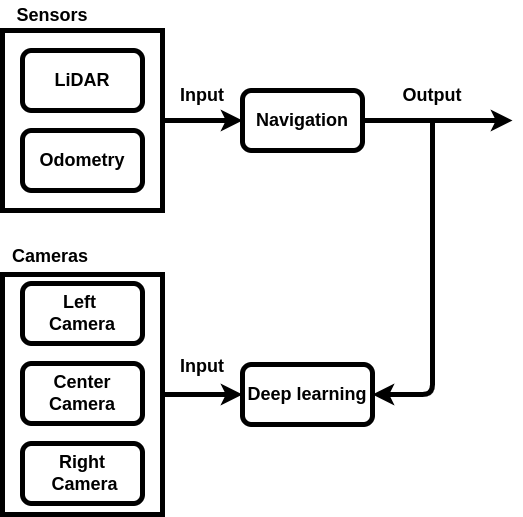
\includegraphics[scale=0.3]{images/old-method1.png}
    \subcaption{Learning phase}
  \end{minipage}
  \begin{minipage}[b]{0.45\linewidth}
    \centering
    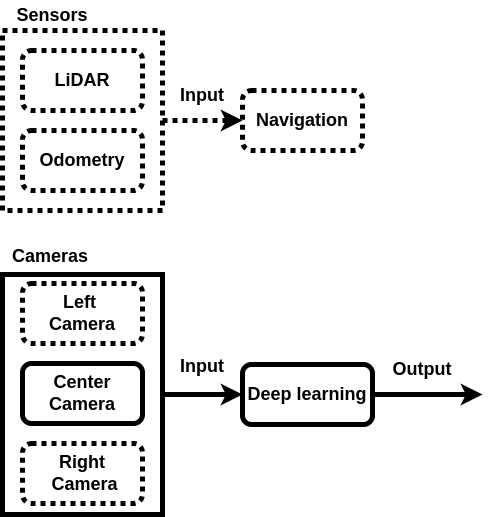
\includegraphics[scale=0.3]{images/old-method2.png}
    \subcaption{Test phase}
  \end{minipage}
  \caption{Conventional method system}
  \label{Fig:conv-method}%\vspace*{-2mm}
\end{figure}

\

